\documentclass[conference]{IEEEtran}
\IEEEoverridecommandlockouts
\usepackage{amsmath,amssymb,amsfonts}
\usepackage{graphicx}
\usepackage{booktabs}
\usepackage{multirow}
\usepackage{siunitx}
\usepackage{xcolor}
\usepackage{cite}
\usepackage[hidelinks]{hyperref}
\sisetup{detect-all, per-mode=symbol, group-minimum-digits=4}
\graphicspath{{figures/}}
\newcommand{\vect}[1]{\boldsymbol{#1}}
\newcommand{\Ns}{\,\si{N.s}}

\begin{document}

\title{Simulation-Based Validation of a Distributed-Thruster Wearable Mobility Suit for Fall Arrest, Boosted Jumping and Balance Recovery}

\author{\IEEEauthorblockN{[Author name]}
\IEEEauthorblockA{\textit{Mobility Suit Simulator Project}\\
\texttt{github.com/CodeShali/CodeShali}, branch \texttt{claude/mobility-suit-simulator-m3e91k}}}

\maketitle

\begin{abstract}
We present a physics simulator and control stack for a wearable mobility suit that uses 44 distributed thrusters (two \SI{1.5}{kN} gas lift pods, two \SI{300}{N} electric fans and forty \SI{40}{N} micro gas jets) to help a \SI{100}{kg} wearer land safely, jump higher and keep balance. The wearer is a 15-segment, 22-joint MuJoCo multibody model; actuators have first-order lag and shared impulse and battery budgets; the controllers see only noisy, delayed IMU, radar-altimeter, foot-pressure and encoder signals through a sensor-only state estimator. A bounded, class-weighted least-squares allocator maps a desired centre-of-mass wrench to thruster forces at \SI{500}{Hz}. Model-based controllers solve three tasks under full domain randomisation (mass $\pm$\SI{10}{\%}, thrust $\pm$\SI{15}{\%}, actuator lag $\pm$\SI{50}{\%}, sensor noise $\times$0.5--2, friction 0.5--1.0): drop landing from 1--5\,m at up to \SI{30}{\degree} tilt and \SI{2}{rad/s} spin succeeds in \SI{99.5}{\%} of 1{,}000 episodes (Wilson 95\,\% CI 98.8--99.8\,\%); a boosted jump onto a \SI{2.5}{m} platform and recovery from a \SI{200}{N}, \SI{0.2}{s} push on a \SI{0.3}{m} beam each succeed in 200/200 episodes, all within the gas and battery budgets. A residual PPO policy trained for 850k steps keeps the landing success rate (\SI{99.4}{\%}) while cutting total gas by \SI{6.3}{\%}. The simulated braking impulse agrees with a first-principles impulse model to within \SI{7}{\%} on average ($r=0.92$). Stress tests and two layout variants show that lateral authority, not lift, limits the design: four extra side jets raise \SI{500}{N}-push survival from \SI{51}{\%} to \SI{90}{\%}, and moving the lift pods \SI{3.6}{cm} forward onto the centre of mass saves \SI{5.9}{\%} of gas without learning.
\end{abstract}

\begin{IEEEkeywords}
wearable robotics, thrust allocation, fall arrest, capture point, state estimation, domain randomization, residual reinforcement learning, MuJoCo
\end{IEEEkeywords}

%=====================================================================
\section{Introduction}
Falls from height and loss of balance are leading causes of injury. A suit that can apply large, fast forces to the whole body could arrest a fall, add impulse to a jump, or catch a stumble. Building such hardware is costly and dangerous, so the first question is whether the idea works at all under realistic physics, sensing and actuator limits. This paper answers that question \emph{in simulation} for one concrete design: a \SI{9}{kg} suit worn by a \SI{91}{kg} person, with 44 push-only thrusters distributed over the body.

The phase-one goal was to show in software that the suit can land a \SI{100}{kg} human safely from 1--5\,m at random body orientations, and to measure what the same hardware can do for jumping and balance. The contributions are:
\begin{enumerate}
\item an open, configurable simulator (MuJoCo~\cite{todorov2012mujoco} + Gymnasium~\cite{towers2024gymnasium}) in which every physical parameter comes from YAML, every experiment is seeded and logged with its configuration and code version, and the controllers can read only simulated sensors;
\item a sensor-only estimator, a real-time constrained thrust allocator, and model-based controllers for drop landing, boosted jumping and push recovery;
\item a statistical evaluation over 3{,}000+ randomised episodes, including a residual reinforcement-learning layer~\cite{silver2018residual,johannink2019residual}, budget accounting, and a first-principles check of the simulated impulse;
\item quantitative hardware recommendations obtained by re-running the unchanged controllers on modified thruster layouts.
\end{enumerate}
Section~\ref{sec:claims} states precisely what these results do and do not establish.

%=====================================================================
\section{System Model}
\label{sec:model}

\subsection{Multibody wearer and suit}
The wearer is a procedurally generated MJCF model of 15 rigid segments (pelvis, torso, head, upper and lower arms, hands, thighs, shanks, feet), \SI{1.80}{m} tall. Segment masses follow de~Leva's fractions~\cite{deleva1996} of \SI{91}{kg} (e.g.\ torso \SI{35.5}{\%}, pelvis \SI{14.2}{\%}, thigh \SI{10.0}{\%}). A free joint on the pelvis gives 6 floating-base degrees of freedom; 22 hinge joints (3 lumbar, neck, 2 per shoulder, elbows, 3 per hip, knees, 2 per ankle) bring the model to $n_q=29$, $n_v=28$. Each hinge has a position servo $\tau = k_p(q^\ast-q) - k_v\dot q$, saturated at a torque limit (e.g.\ knee $k_p=\SI{1200}{N.m/rad}$, $k_v=\SI{60}{N.m.s/rad}$, $|\tau|\le\SI{400}{N.m}$), plus passive damping at hips, knees and ankles that absorbs landing energy. The servos hold a landing-ready posture (knees \SI{20}{\degree}, hips and ankles \SI{10}{\degree}); they stand for the wearer's muscles, not for a muscle model. The \SI{9}{kg} suit is attached as mass-only geometry: \SI{3}{kg} of hip pods and tanks on the pelvis, a \SI{1.5}{kg} tube frame and \SI{2}{kg} shell spread over the torso and limbs, \SI{1.5}{kg} of airbags and \SI{1}{kg} of compute on the torso. The compiled model weighs \SI{100.000}{kg}. Body geometries collide with the ground but not with each other.

The equations of motion are the standard constrained multibody form
\begin{equation}
M(q)\dot v + c(q,v) = S^{\top}\tau_{\text{servo}} + \sum_{i} J_i^{\top}(q)\,\vect f_i + J_c^{\top}\vect\lambda,
\label{eq:eom}
\end{equation}
where $\vect f_i$ are thruster forces applied at their mount sites, $J_i$ the site Jacobians and $\vect\lambda$ the contact impulses solved by MuJoCo's soft-contact model~\cite{todorov2012mujoco}. Integration uses the implicit-fast integrator with a \SI{1}{ms} step. Aerodynamic drag is modelled as a single whole-body term $\vect F_d=-\tfrac12\rho C_d A\,|\vect v|\vect v$ with $\rho=\SI{1.225}{kg/m^3}$, $C_d=1.0$, $A=\SI{0.7}{m^2}$, applied at the centre of mass (CoM).

Three airbags (collar, chest, hips) are compiled as compliant contact geometries (soft \texttt{solref}/\texttt{solimp}) that are stowed inside the body and inflate linearly over \SI{30}{ms} when commanded. In a face-down \SI{0.5}{m} test drop, a deployed chest bag lowered the peak torso specific force from 266 to \SI{89}{m/s^2}.

\subsection{Actuators}
Table~\ref{tab:act} lists the 44 thrusters. Each has a fixed mount site and a fixed nozzle direction $\hat{\vect d}_i$ on its segment and can only push. Each follows a first-order lag discretised with forward Euler,
\begin{equation}
f_i^{k+1} = f_i^{k} + \alpha_i\,(u_i^{k}-f_i^{k}),\qquad \alpha_i=\min(\Delta t/\tau_i,\,1),
\label{eq:lag}
\end{equation}
with command and output clamped to $[0,u_{\max,i}]$. Gas thrusters draw $\sum_i f_i\,\Delta t$ from a shared tank per class; when a step would overdraw a tank, all its thrusters are scaled so that the tank reaches exactly zero, after which $u_{\max,i}=0$. The fans draw battery power $P=k f^{1.5}$ with $k$ fitted so that \SI{300}{N} costs \SI{1.2}{kW} ($k=\SI{0.231}{W.N^{-1.5}}$).

\begin{table}[t]
\centering
\caption{Thruster classes (nominal values; randomised per episode)}
\label{tab:act}
\setlength{\tabcolsep}{3.2pt}
\begin{tabular}{@{}lrrrl@{}}
\toprule
Class & Count & $f_{\max}$ & $\tau$ & Budget \\
\midrule
Lift gas pod (hips, $+z$) & 2 & \SI{1500}{N} & \SI{5}{ms} & \SI{2500}{N.s} shared \\
Electric fan (hips, $+z$) & 2 & \SI{300}{N} & \SI{100}{ms} & \SI{150}{Wh} battery \\
Micro gas jet (8 regions) & 40 & \SI{40}{N} & \SI{5}{ms} & \SI{600}{N.s} shared \\
\bottomrule
\end{tabular}
\vspace{2pt}

\footnotesize Jets sit at shoulders (6), upper arms (4), wrists (6), upper back (6), lower back (4), thighs (6), calves (4) and heels (4), pointing forward, backward, up or sideways.
\end{table}

\subsection{Sensors}
Every segment carries an IMU (accelerometer $\sigma=\SI{0.05}{m/s^2}$, gyro $\sigma=\SI{0.01}{rad/s}$, \SI{2}{ms} delay). A radar altimeter on the pelvis points along the body's $-z$ axis (range noise \SI{2}{\%} of range, \SI{5}{ms} delay); its ray ignores the wearer's own geometry. Both soles have pressure sensors (\SI{5}{\%}, \SI{1}{ms}), all hinges have encoders (\SI{0.002}{rad}, \SI{1}{ms}) and every thruster reports its force exactly. Delays are implemented with per-sensor ring buffers at the physics rate; noise is drawn at read time from the episode's seeded generator. EMG intent sensing is an interface stub.

\subsection{Domain randomisation}
Following domain randomisation~\cite{tobin2017dr}, each episode draws: human segment masses $\times U(0.9,1.1)$; per-thruster $f_{\max}\times U(0.85,1.15)$ and $\tau\times U(0.5,1.5)$; a sensor-noise scale $U(0.5,2)$; ground friction $U(0.5,1.0)$. For drop landing it also draws the drop height (feet above ground) $U(1,5)$\,m, an initial tilt of up to \SI{30}{\degree} about a random horizontal axis, a random yaw, and an initial angular velocity $U(-2,2)$\,\si{rad/s} per axis. The controllers use a nominal \SI{100}{kg} mass and never see the drawn values.

%=====================================================================
\section{State Estimation}
\label{sec:est}
Controllers run at \SI{500}{Hz} and read only the estimator output: CoM height and velocity, the lowest sole's height, torso attitude and rate, joint angles, foot contact, remaining budgets and a free-fall flag. MuJoCo ground truth is used only to seed the estimator at $t=0$, with errors added (\SI{2}{\degree} attitude, \SI{0.05}{m/s}, \SI{0.05}{m}), standing for an alignment done before the fall.

\paragraph*{Attitude} The torso quaternion is propagated by integrating the gyro. When the body is quasi-static ($\big|\|\vect a_{\text{IMU}}\|-g\big|<\SI{0.4}{m/s^2}$ and $\|\vect\omega\|<\SI{0.3}{rad/s}$) a complementary term with gain \SI{2}{s^{-1}} pulls the estimated gravity direction toward the measured one. This corrects tilt only; yaw is unobservable and irrelevant to the tasks.

\paragraph*{Kinematics} A private \texttt{MjData} is posed from the estimated torso attitude and the measured joint angles. Forward kinematics then gives the CoM, each segment's orientation, the sole and altimeter poses, and every thruster's position and direction relative to the CoM.

\paragraph*{CoM acceleration} An accelerometer measures specific force $\vect a_s = R^{\top}(\ddot{\vect p}-\vect g)$. For each IMU $j$, the lever-arm term $\vect\omega\times(\vect\omega\times\vect r_j)$ is removed using its own gyro, the reading is rotated to the world frame with the segment's estimated orientation $\hat R_j$, and the readings are averaged with mass weights $m_j$ (each body's mass lumped onto the nearest IMU-carrying ancestor):
\begin{equation}
\hat{\ddot{\vect p}}_{\text{CoM}} = \frac{1}{\sum_j m_j}\sum_j m_j\,\hat R_j\,\vect a_{s,j} + \vect g .
\label{eq:comacc}
\end{equation}
In free fall every $\vect a_{s,j}=0$, so \eqref{eq:comacc} returns exactly $\vect g$ whatever the attitude error. This is what keeps velocity estimates accurate through a tumbling fall.

\paragraph*{Vertical channel} A two-state Kalman filter on $[h, v_z]$ is driven by the vertical component of \eqref{eq:comacc}. The measurement is the altimeter slant range $r$ projected with the estimated attitude, $h_{\text{meas}}=r\cos\theta_{\text{inc}}+\Delta h_{\text{kin}}+v_z\,t_d$, where $\Delta h_{\text{kin}}$ moves the reference from the sensor to the CoM and $t_d=\SI{5}{ms}$ compensates the delay. Measurement variance grows with incidence angle, because attitude error biases the projection. Rays beyond \SI{60}{\degree} incidence are ignored and innovations beyond $5\sigma$ are gated. If such innovations persist for \SI{0.1}{s}, the filter adopts the new surface, which lets it track a platform or beam.

\paragraph*{Fall detection} Free fall is latched when either the torso specific force or the CoM specific force from \eqref{eq:comacc} stays below \SI{2}{m/s^2} for \SI{50}{ms}. The CoM test is needed for spinning bodies: at 2--3\,\si{rad/s} the torso IMU's centripetal term alone stays above the threshold, which delayed detection by up to \SI{0.5}{s} or prevented it altogether before this fix.

\paragraph*{Measured accuracy} On 3\,m drops with \SI{20}{\degree} tilt and \SI{1}{rad/s} spin (8 seeds, configured noise and seeding errors), the worst attitude error was \SI{2.2}{\degree} (essentially the \SI{2}{\degree} seeding error), vertical-velocity error \SI{0.08}{m/s} and height error \SI{0.052}{m}. Free fall was detected at \SI{52}{ms} in every case, including spinning drops. One update takes about \SI{0.1}{ms}.

%=====================================================================
\section{Thrust Allocation}
\label{sec:alloc}
Controllers command a wrench $\vect w=[\vect F;\vect\tau]\in\mathbb R^6$ about the estimated CoM in a world-aligned frame. Because limbs move, the allocation matrix is rebuilt every control step from the estimated thruster geometry:
\begin{equation}
A = \begin{bmatrix}\hat{\vect d}_1 & \cdots & \hat{\vect d}_N\\ \vect r_1\times\hat{\vect d}_1 & \cdots & \vect r_N\times\hat{\vect d}_N\end{bmatrix}\in\mathbb R^{6\times N}.
\end{equation}
With $S=\mathrm{diag}(f_{\max,i}^{\text{nom}})$ and normalised commands $\vect v=S^{-1}\vect u$, we solve
\begin{equation}
\min_{\vect v}\ \|W(AS\vect v-\vect w)\|^2+\rho\sum_i\lambda_i v_i^2\quad\text{s.t.}\quad 0\le v_i\le u_{\max,i}/s_i,
\label{eq:alloc}
\end{equation}
where $W=\mathrm{diag}(1,1,1,L^{-1},L^{-1},L^{-1})$ with $L=\SI{0.3}{m}$ puts torques on the same scale as forces. The class weights $\lambda$ (pods $10^{-2}$, fans $3\cdot10^{-2}$, jets $10^{-1}$) make the pods carry large vertical force and the well-levered jets carry torque. Because the regulariser is tiny relative to tracking in \si{N^2}, feasible wrenches are reproduced almost exactly. Problem~\eqref{eq:alloc} is a bounded least-squares problem~\cite{stark1995bvls,johansen2013allocation}. We solve it with a warm-started primal active-set method that matches SciPy's BVLS to $10^{-13}$ relative objective, in \SI{0.52}{ms} per call (BVLS: \SI{1.6}{ms}).

\paragraph*{Authority} At the nominal pose $A$ has rank 6 (singular values 5.15 to 0.79). Linear programs over the bounded thrust set give the achievable torque per axis with the other wrench components held fixed (Table~\ref{tab:auth}). Roll authority without lift is only \SI{\pm27}{N.m}, because no upward thruster may fire when $F_z=0$, leaving the four side jets. With hover lift, differential pod thrust raises it to \SI{\pm225}{N.m}. A second geometric fact matters later: the pods sit \SI{3.6}{cm} behind the whole-body CoM, so braking thrust creates a pitch moment that the jets must cancel.

\begin{table}[t]
\centering
\caption{Torque authority at the nominal pose [N\,m]}
\label{tab:auth}
\begin{tabular}{@{}lccc@{}}
\toprule
Condition & Roll $\tau_x$ & Pitch $\tau_y$ & Yaw $\tau_z$\\
\midrule
Pure torque ($\vect F=0$) & $\pm 26.8$ & $-225.6/+182.4$ & $\pm 65.3$ \\
Hovering ($F_z=mg$) & $\pm 224.6$ & $-225.6/+296.4$ & $\pm 69.7$ \\
\bottomrule
\end{tabular}
\end{table}

%=====================================================================
\section{Controllers}
\label{sec:ctrl}

\subsection{Drop landing (T1)}
The landing controller treats the body like a quadrotor~\cite{lee2010geometric,mellinger2011minimum}: the summed pod axis $\hat{\vect z}_p$ is the thrust direction.

\emph{Phase 1 (detect).} The controller waits for the free-fall latch, or for an estimated descent faster than \SI{0.4}{m/s} without foot contact.

\emph{Phase 2 (attitude).} A desired thrust axis is computed from the desired force (gravity compensation plus horizontal-velocity damping $-k_h\vect v_{xy}$, $k_h=\SI{2}{s^{-1}}$) and limited to \SI{10}{\degree} from vertical. The axis-angle error $\vect e$ between $\hat{\vect z}_p$ and the desired axis (yaw ignored) drives a torque command. The commanded rate is the smaller of a PD law ($k_p\approx2600$, $k_d\approx\SI{380}{N.m.s/rad}$) and the time-optimal $\sqrt{2\alpha_{\max}|e|}$ law with $\alpha_{\max}=\SI{8}{rad/s^2}$; yaw rate is damped. When roll demand exceeds the jets' roughly \SI{40}{N.m}, extra pod thrust is requested so that the allocator can roll the body differentially.

\emph{Phase 3 (braking).} With feet height $h$ and descent speed $v=-\dot h$, the vertical velocity reference is the constant-deceleration profile
\begin{equation}
v_{\text{ref}}(h) = \sqrt{v_t^2 + 2a\,(h-h_t)},\qquad h>h_t,
\label{eq:profile}
\end{equation}
with $v_t=\SI{1.2}{m/s}$ at $h_t=\SI{0.3}{m}$ and $a=\SI{9}{m/s^2}$, held at $v_t$ below $h_t$. Thrust starts only when $v$ reaches $v_{\text{ref}}$, which is the latest possible moment and therefore minimises the gravity loss. The vertical force is $F_z=m_{\text{nom}}\big(g+a_{\text{ff}}+k_v(v-v_{\text{ref}})\big)$ with $k_v=\SI{8}{s^{-1}}$. It is applied as $T\hat{\vect z}_p$, so the request is always achievable by the pods.

\emph{Phase 4 (touchdown).} Thrust is cut at foot contact or $h<\SI{5}{cm}$. Airbags deploy if the predicted impact speed exceeds \SI{2.5}{m/s} or the body is tilted more than \SI{45}{\degree} near the ground.

\subsection{Boosted jump (T2)}
The jump controller settles for \SI{0.8}{s} (letting the gravity-based tilt correction converge), crouches, then extends the legs while pods and fans deliver about \SI{2.9}{kN}. The burn stops when the predicted ballistic apex of the soles is \SI{0.63}{m} above the platform. Flight uses jet-only horizontal guidance. Descent reuses \eqref{eq:profile} relative to the platform top, with guards that keep the toes behind the near edge until the soles clear it. Since the estimator gives no horizontal position, the controller integrates its velocity estimate. It corrects that estimate when the altimeter re-acquires the platform: this event marks the edge crossing, giving both a position fix and a velocity-bias estimate. That correction raised success in development runs from 27/40 to 80/80.

\subsection{Push recovery on a beam (T3)}
The balance controller uses the linear inverted pendulum~\cite{kajita2001lipm} and the instantaneous capture point~\cite{pratt2006capture}
\begin{equation}
\vect\xi=\vect c+\dot{\vect c}/\omega_0,\qquad \omega_0=\sqrt{g/z_0},
\label{eq:cp}
\end{equation}
where $\vect c$ is the CoM relative to the feet (from kinematics) and $z_0\approx\SI{1.05}{m}$. With thruster acceleration $\vect u$ added, the CoM obeys $\ddot{\vect c}=\omega_0^2(\vect c-\vect p)+\vect u$, with $\vect p$ the centre of pressure, so the capture point evolves as
\begin{equation}
\dot{\vect\xi}=\omega_0(\vect\xi-\vect p)+\vect u/\omega_0 .
\label{eq:cpdyn}
\end{equation}
The controller asks for $\dot{\vect\xi}=-3\vect\xi$. The feet supply $\vect p$ as long as it lies inside the foot polygon shrunk by \num{0.04}/\SI{0.03}{m}; only the excess is requested from the thrusters, as a moment about the feet ($u_x=(F_x+\tau_y/h)/m$, $u_y=(F_y-\tau_x/h)/m$). Quiet standing therefore uses no gas.

\subsection{Residual reinforcement learning}
A PPO~\cite{schulman2017ppo} policy (Stable-Baselines3~\cite{raffin2021sb3}, MLP $128\times128$) acts at \SI{50}{Hz}. It outputs a residual wrench in $[-1,1]^6$, scaled to \SI{\pm300}{N} horizontal, \SI{\pm600}{N} vertical and \SI{\pm60}{}/\SI{30}{N.m}, which is added to the T1 baseline wrench before allocation. The observation (53 values) is built from estimator outputs only. The final layer is zero-initialised, so the untrained policy reproduces the baseline exactly (verified bit-for-bit). The reward follows the specification: $+10$ for a safe landing, $-k_1 v_{\text{imp}}^2$, $-k_2\theta_{\text{imp}}$, $-50$ for head or torso contact first. The impulse term is applied densely (\SI{0.004}{} per \si{N.s}) and a margin penalty discourages approaching the safety limits. Training ran 450k steps from scratch plus 450k steps warm-started from the 400k checkpoint (850k in total), with 4 environments, using seeds disjoint from the test seeds.

%=====================================================================
\section{Experimental Method}
\label{sec:method}
\paragraph*{Tasks and pass criteria} A T1 landing is \emph{safe} if, at first foot contact, the vertical CoM speed is under \SI{2}{m/s}, the horizontal speed under \SI{1}{m/s}, the torso tilt under \SI{20}{\degree}, and no head, torso or pelvis contact occurred first. All are computed from MuJoCo ground truth. T2 succeeds if the first contact after lift-off is a foot on the platform top, the same three limits hold at that contact, and the wearer is still standing on the platform \SI{1}{s} later; the platform is \SI{2.5}{m} high and $1.5\pm0.2$\,m away. T3 succeeds if, after \SI{4}{s}, both soles are on the beam, the pelvis is upright and torso tilt is under \SI{30}{\degree}. The push is \SI{200}{N} for \SI{0.2}{s} in a uniformly random horizontal direction at a random time between 0.5 and \SI{1.5}{s}. T4 requires every episode to stay within every budget. Targets: T1~$\ge\SI{95}{\%}$, T2~$\ge\SI{90}{\%}$, T3~$\ge\SI{95}{\%}$.

\paragraph*{Statistics} Episode $i$ uses seed $i$, so different controllers and layouts face identical initial states and randomisation draws, and differences are \emph{paired}. Success rates carry Wilson score intervals~\cite{wilson1927}. Paired differences are reported as mean $\pm$ 95\,\% half-width.

\paragraph*{Reproducibility} Physics \SI{1}{ms}, control \SI{2}{ms}, episodes capped at \SI{5}{s}. Every run stores its full configuration and git hash. The 134 unit and integration tests pass. Each evaluation re-renders its 5 worst and 5 best episodes to video.

%=====================================================================
\section{Results}
\label{sec:results}

\subsection{Component verification (M1--M3)}
Table~\ref{tab:verif} lists the checks that establish the building blocks behave as modelled. The allocation test generates feasible wrenches as $\vect w=A\vect u_{\text{true}}$ with $\vect u_{\text{true}}$ uniform in the bounds, under random global rotations. The 2\,\% requirement is met with a worst error of $3\times10^{-8}$.

\begin{table}[t]
\centering
\caption{Component verification (selected automated tests)}
\label{tab:verif}
\setlength{\tabcolsep}{3pt}
\begin{tabular}{@{}p{3.6cm}p{2.0cm}p{2.2cm}@{}}
\toprule
Check & Requirement & Measured \\
\midrule
Total model mass & $100\pm0.5$\,kg & \SI{100.000}{kg} \\
Thruster sites, IMUs & 44, 15 & 44, 15 \\
Torso accel.\ in free fall & $\approx 0$ & $<10^{-3}$\,\si{m/s^2} \\
Lag after one $\tau$ (Euler, $\Delta t/\tau=0.2$) & $1-(0.8)^5$ & \SI{67.2}{\%} \\
Fan power at \SI{300}{N} & \SI{1.2}{kW} & \SI{1200}{W} \\
Shared-budget exhaustion & output $=0$, no overdraw & exact to last step \\
Allocation, 200 random feasible wrenches & error $\le\SI{2}{\%}$ & max $3.4\times10^{-8}$ \\
Pure torque request & jets only & pods, fans $=0$ \\
Estimator attitude (3\,m, \SI{20}{\degree}, 1\,rad/s) & $<\SI{3}{\degree}$ & \SI{2.2}{\degree} max \\
Estimator $v_z$ / height & $<0.3$\,m/s / 0.15\,m & 0.08\,m/s / 0.052\,m \\
Free-fall detection (incl.\ spin) & 50--80\,ms & \SI{52}{ms} \\
Zero residual $=$ baseline & identical episode & bit-identical \\
\bottomrule
\end{tabular}
\end{table}

\subsection{Physical consistency: simulated vs.\ first-principles impulse}
A simple impulse model predicts how much gas the baseline should use. Under profile~\eqref{eq:profile} the body falls freely until its speed meets the profile at height
\begin{equation}
h_b=\frac{2gH-v_t^2+2a\,h_t}{2(g+a)},\qquad v_0=\sqrt{2g(H-h_b)},
\label{eq:hb}
\end{equation}
for release height $H$. It then decelerates at $a$ with thrust $m(g+a)$ for $(v_0-v_t)/a$ seconds and holds $v_t$ for $h_t/v_t$ seconds, so the ideal impulse is
\begin{equation}
I^\star(H)=m\,(v_0-v_t)\Big(1+\frac{g}{a}\Big)+m\,g\,\frac{h_t}{v_t}.
\label{eq:impulse}
\end{equation}
The factor $(1+g/a)=2.09$ is the gravity loss of braking at \SI{9}{m/s^2}. At $H=\SI{3}{m}$, \eqref{eq:hb}--\eqref{eq:impulse} give $h_b=\SI{1.67}{m}$, $v_0=\SI{5.11}{m/s}$ and $I^\star=\SI{1062}{N.s}$, against \SI{1019}{N.s} measured in the fixed 3\,m upright drop. Over the 1{,}000 randomised episodes, with $m$ set to each episode's drawn mass, the simulated pod impulse is $1.07\times I^\star$ on average (5th--95th percentile 0.91--1.26) with correlation $r=0.92$ (Fig.~\ref{fig:theory}, Table~\ref{tab:theory}). The roughly \SI{7}{\%} excess is consistent with thrust spent on tilted axes, feedback corrections, roll-assist thrust and actuator lag. This agreement indicates that the contact, gravity, thrust and budget bookkeeping in the simulator are mutually consistent. It checks consistency; it does not validate the model against real hardware.

\begin{figure}[t]
\centering
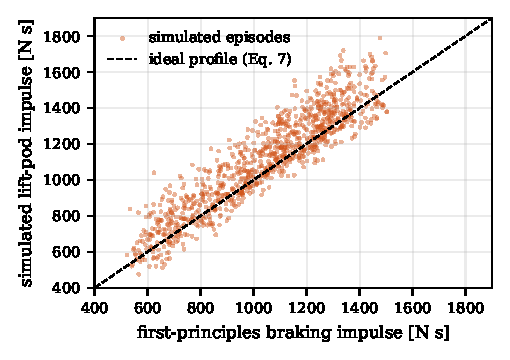
\includegraphics[width=\columnwidth]{theory_vs_sim.pdf}
\caption{Simulated lift-pod impulse per T1 episode vs.\ the ideal braking impulse of Eq.~\eqref{eq:impulse} (1{,}000 randomised drops, baseline controller).}
\label{fig:theory}
\end{figure}

\begin{table}[t]
\centering
\caption{Ideal vs.\ simulated pod impulse by drop height (baseline, 1{,}000 episodes)}
\label{tab:theory}
\begin{tabular}{@{}lrrrr@{}}
\toprule
$H$ bin [m] & $n$ & $\bar H$ [m] & $I^\star$ [N\,s] & Simulated [N\,s] \\
\midrule
1--2 & 258 & 1.49 & 714 & $773\pm130$ \\
2--3 & 217 & 2.53 & 961 & $1029\pm120$ \\
3--4 & 263 & 3.48 & 1152 & $1221\pm115$ \\
4--5 & 262 & 4.56 & 1324 & $1405\pm123$ \\
\bottomrule
\end{tabular}
\end{table}

\subsection{T1: drop landing}
\begin{figure*}[t]
\centering
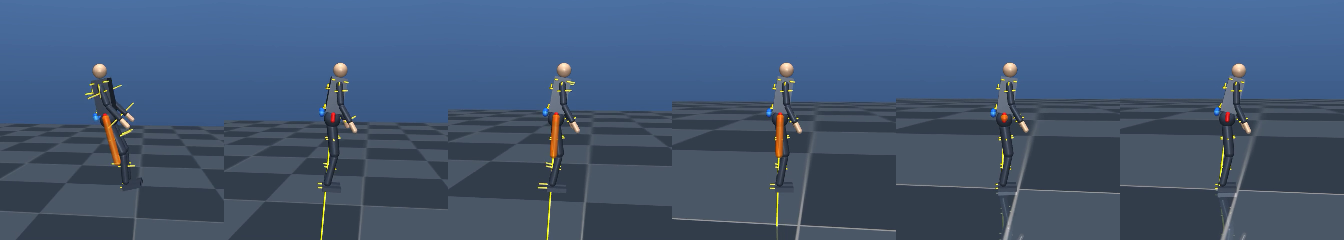
\includegraphics[width=\textwidth]{strip_t1.png}\\[2pt]
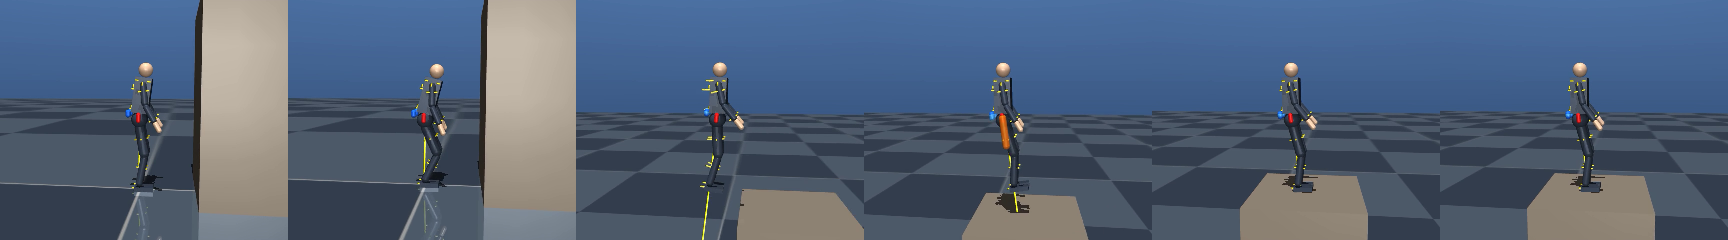
\includegraphics[width=\textwidth]{strip_t2.png}\\[2pt]
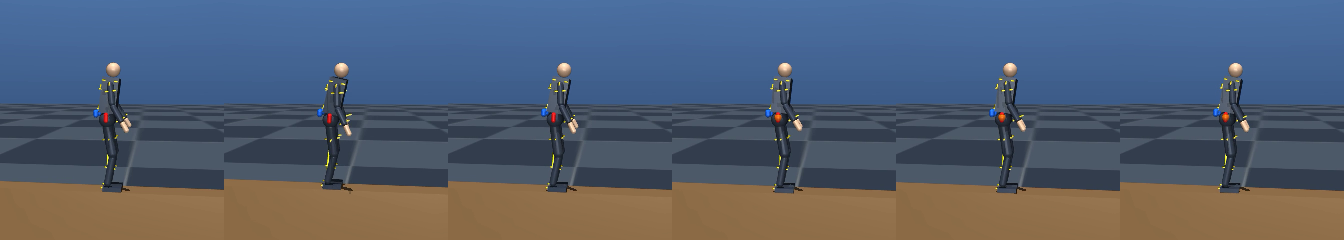
\includegraphics[width=\textwidth]{strip_t3.png}
\caption{Simulated episodes, left to right in time. Top: T1, 5\,m drop starting \SI{23}{\degree} tilted (lands at \SI{1.43}{m/s} vertical, \SI{0.29}{m/s} horizontal, \SI{7.7}{\degree} tilt; with thrust disabled the same drop hits the ground arm-first at \SI{10.4}{m/s}). Middle: T2, crouch, leg push with pod boost, flight, braking onto the \SI{2.5}{m} platform. Bottom: T3, a \SI{200}{N} push \SI{72}{\degree} off the beam axis, recovered with jets. Yellow lines are thruster plumes, with length proportional to force.}
\label{fig:strips}
\end{figure*}

The fixed 3\,m upright drop (milestone M4) lands safely in 20/20 runs, at \SI{1.47}{m/s} vertical, \SI{0.27}{m/s} horizontal and \SI{7.8}{\degree} tilt. On the full randomised task the baseline is safe in \textbf{995/1000} episodes (Table~\ref{tab:main}). At impact, vertical speed averages \SI{1.48}{m/s} (max 1.67), horizontal \SI{0.34}{m/s} (p95 0.58) and tilt \SI{7.4}{\degree} (max 18.2). A foot touches first in every episode and no airbag is deployed. All five failures are horizontal-speed violations (1.05--1.83\,\si{m/s}) in short drops (1.0--1.65\,m) that start with large tilt (\SI{23}{}--\SI{27}{\degree}) and spin (2.4--3.2\,\si{rad/s}). Success is 100\,\% above 2\,m and 97.6--98.5\,\% below. The mechanism is time: a 1.5\,m fall lasts about \SI{0.5}{s}, most of which the attitude loop spends righting the thrust axis. The horizontal velocity created while braking on a tilted axis cannot then be removed, because horizontal damping comes only from tilting the pod axis (limited to \SI{10}{\degree}) and the jets' direct lateral force is small.

\begin{table}[t]
\centering
\caption{Acceptance results (Wilson 95\,\% CI)}
\label{tab:main}
\setlength{\tabcolsep}{2.5pt}
\begin{tabular}{@{}llrcc@{}}
\toprule
Task & Controller & $n$ & Success & Target\\
\midrule
T1 drop & baseline & 1000 & \textbf{99.5\,\%} [98.8, 99.8] & $\ge$95\,\%\\
T1 drop & baseline + residual PPO & 1000 & \textbf{99.4\,\%} [98.7, 99.7] & $\ge$95\,\%\\
T2 jump & baseline & 200 & \textbf{100\,\%} [98.1, 100] & $\ge$90\,\%\\
T3 push & baseline & 200 & \textbf{100\,\%} [98.1, 100] & $\ge$95\,\%\\
T4 budgets & all of the above & 2400 & \textbf{100\,\%} within & 100\,\%\\
\bottomrule
\end{tabular}
\end{table}

\subsection{Residual reinforcement learning (M5)}
On the same 1{,}000 seeds (Table~\ref{tab:rl}), the residual policy's success rate is statistically indistinguishable from the baseline's. It fails three seeds the baseline passes and passes two the baseline fails. Total gas falls by $88.6\pm3.0$\,\si{N.s} (\SI{-6.3}{\%}), and it is lower in 96\,\% of episodes. The policy does this by braking later and landing faster: mean vertical impact rises from 1.48 to \SI{1.74}{m/s} (p95 1.91, still under 2.0), and less pod thrust means slightly more jet use. It did not remove the low-drop horizontal failures. The training curve (Fig.~\ref{fig:train}) was still improving at 850k steps. The specified 20M-step run would take an estimated 37--43\,h at the measured 130--150 steps/s on four CPU cores.

\begin{table}[t]
\centering
\caption{Baseline vs.\ residual PPO, paired over seeds 0--999}
\label{tab:rl}
\setlength{\tabcolsep}{3pt}
\begin{tabular}{@{}lrrr@{}}
\toprule
Quantity & Baseline & Residual & Paired diff.\\
\midrule
Safe landings & 995 & 994 & n.s.\\
Total gas [N\,s] & 1410 & 1322 & $-88.6\pm3.0$ ($-6.3\,\%$)\\
Pod gas [N\,s] & 1112 & 1015 & $-97.0\pm2.4$ ($-8.7\,\%$)\\
Jet gas [N\,s] & 298 & 307 & $+8.4\pm2.6$ ($+2.8\,\%$)\\
$|v_z|$ at impact [m/s] & 1.48 & 1.74 & $+0.26\pm0.005$\\
Tilt at impact [deg] & 7.42 & 6.87 & $-0.55\pm0.07$\\
\bottomrule
\end{tabular}
\end{table}

\begin{figure}[t]
\centering
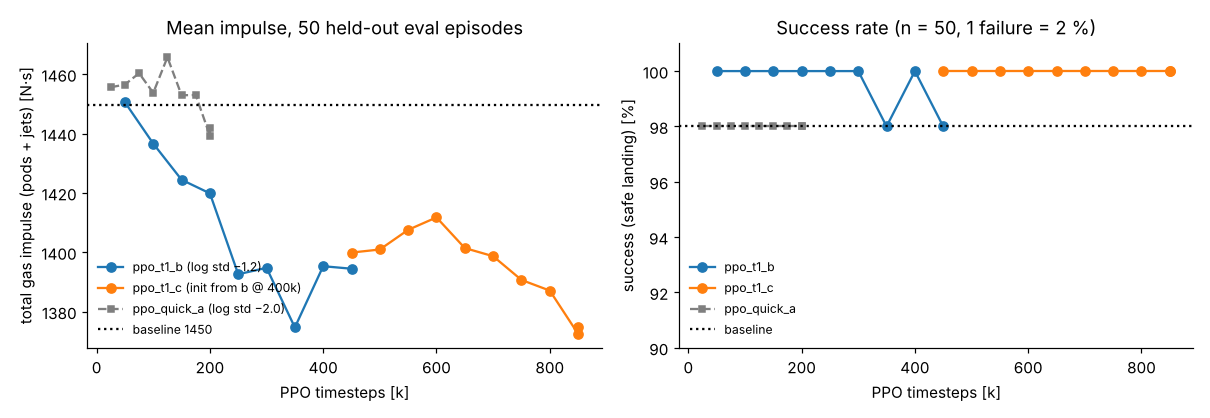
\includegraphics[width=\columnwidth]{training_curve.png}
\caption{Residual PPO training: periodic deterministic evaluation on 50 held-out episodes (total impulse and success vs.\ environment steps); dotted: baseline on the same episodes.}
\label{fig:train}
\end{figure}

\subsection{T2: boosted jump}
All 200 jumps land on the platform and stay there. At platform contact, vertical speed averages \SI{1.09}{m/s} (max 1.29), horizontal \SI{0.21}{m/s} (max 0.46) and tilt \SI{3.0}{\degree} (max 4.3). A ballistic estimate explains the gas use. Raising the soles \SI{3.13}{m} needs a take-off speed of $\sqrt{2g\cdot3.13}=\SI{7.8}{m/s}$. With about \SI{2.9}{kN} of thrust the net acceleration is about \SI{19}{m/s^2}, so the burn lasts about \SI{0.41}{s} and costs about \SI{1.2}{kN.s} if thrust alone does the work. The measured pod impulse is \SI{1130}{N.s} on average, which includes the descent braking. The leg push saves roughly \SI{225}{N.s}: without it, pod use rises to \SI{1356}{N.s}. Jet gas, at \SI{482}{N.s} of \SI{600}{N.s} on average, is the binding budget. One episode emptied the jet tank and still succeeded, because the allocator then routes attitude torque through differential pod thrust.

\subsection{T3: push recovery and stress tests}
All 200 nominal pushes are recovered, with \SI{81}{N.s} of jet gas on average and almost no pod gas. Without the controller, 0/100 succeed. Equations~\eqref{eq:cp}--\eqref{eq:cpdyn} explain where the limit lies. A push of impulse $J$ adds $\Delta v=J/m$ to the CoM and moves the capture point by $\Delta\xi=\Delta v/\omega_0$, with $\omega_0=\sqrt{9.81/1.05}=\SI{3.06}{s^{-1}}$. The usable centre-of-pressure range across the beam is $p_{\max}\approx\SI{0.11}{m}$ (\SI{0.15}{m} half-width less margin). From \eqref{eq:cpdyn}, the thrusters must supply at least
\begin{equation}
u_{\min}\approx\omega_0^2\,(\Delta\xi-p_{\max})
\label{eq:umin}
\end{equation}
to keep $\xi$ from running away. For sideways pushes, Table~\ref{tab:stress} compares this with the measured lateral authority: about \SI{1.25}{m/s^2} from jets alone with the default layout, and about \SI{2.2}{m/s^2} with four extra side jets. The success rates follow the predicted margin: no thrust needed at \SI{200}{N}; a borderline case at \SI{400}{N}, where the default suit drops to 88\,\%; and too little authority at \SI{500}{N} (51\,\%, Fig.~\ref{fig:stress}), where every default-suit failure is a push more than \SI{45}{\degree} off the beam axis and ends with the jet tank empty. This is a quasi-static, impulsive-push approximation (the real push lasts \SI{0.2}{s} and pods add some lateral authority through differential thrust), so it predicts trends, not exact rates.

\begin{table}[t]
\centering
\caption{T3 push magnitude: capture-point demand vs.\ success (sideways pushes dominate failures)}
\label{tab:stress}
\setlength{\tabcolsep}{2.4pt}
\begin{tabular}{@{}rrrrcc@{}}
\toprule
Push & $\Delta v$ & $\Delta\xi$ & $u_{\min}$ (Eq.~\ref{eq:umin}) & Default suit & +4 side jets\\
\midrule
\SI{200}{N} & 0.40 & 0.13 & \SI{0.2}{m/s^2} & 100\,\% (200) & 100\,\% (200)\\
\SI{400}{N} & 0.80 & 0.26 & \SI{1.4}{m/s^2} & 88\,\% (100) & 100\,\% (100)\\
\SI{500}{N} & 1.00 & 0.33 & \SI{2.0}{m/s^2} & 51\,\% (100) & 90\,\% (100)\\
\bottomrule
\end{tabular}
\vspace{2pt}

\footnotesize Units: $\Delta v$ in m/s, $\Delta\xi$ in m. Lateral jet authority: default $\approx$1.25, variant $\approx$2.2\,m/s$^2$.
\end{table}

\begin{figure}[t]
\centering
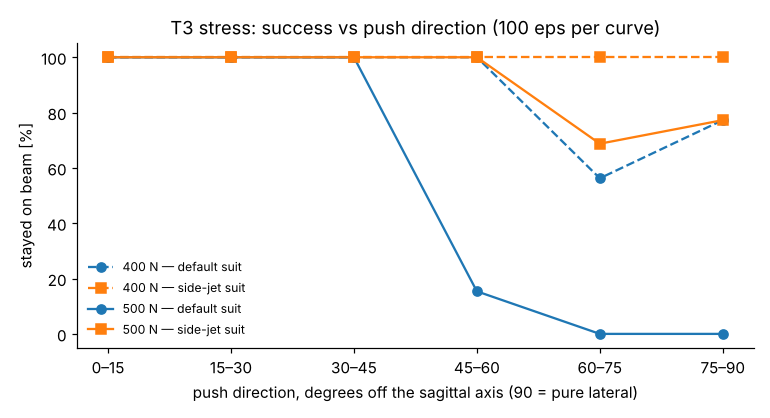
\includegraphics[width=\columnwidth]{t3_stress_by_direction.png}
\caption{T3 stress tests: success vs.\ push direction (degrees off the beam's long axis) for the default and side-jet layouts.}
\label{fig:stress}
\end{figure}

\subsection{T4: budgets}
No episode in any evaluation exceeded a budget (Table~\ref{tab:budget}). The lift pods never used more than \SI{73}{\%} of their tank in any T1 episode, and fans used under \SI{0.3}{Wh} of \SI{150}{Wh}. The jet tank is the binding resource: it averages 80\,\% in T2 and is emptied in \SI{400}{}--\SI{500}{N} pushes. Much of the jet gas in T1 goes to cancelling the pod pitch moment.

\begin{table}[t]
\centering
\caption{Mean (max) consumption per episode}
\label{tab:budget}
\setlength{\tabcolsep}{3pt}
\begin{tabular}{@{}lrrr@{}}
\toprule
Evaluation & Pods [N\,s] & Jets [N\,s] & Fans [Wh]\\
 & /2500 & /600 & /150\\
\midrule
T1 baseline & 1112 (1789) & 298 (600) & 0.01 (0.09)\\
T1 residual & 1015 (1823) & 307 (600) & 0.01 (0.10)\\
T2 jump & 1130 (1221) & 482 (600) & 0.08 (0.10)\\
T3 push 200\,N & 0.3 (6) & 81 (222) & 0.00\\
\bottomrule
\end{tabular}
\end{table}

\subsection{Layout variants}
Both variants reuse the unchanged controllers; the allocator simply picks up the new thruster columns.
\paragraph*{+4 side jets (48 thrusters)} One \SI{40}{N} jet per side at the shoulders and one per side at the hips. In T3 the variant gives the results of Table~\ref{tab:stress}, and at \SI{200}{N} it cuts jet gas by $26.1\pm5.0$\,\si{N.s} (\SI{-32}{\%}). In T1 (200 paired seeds) success is unchanged (198/200) and the same short-drop seeds fail, now only just above the limit (1.04 and \SI{1.01}{m/s}). This confirms that those failures are limited by how fast the body can be righted, not by lateral thrust.
\paragraph*{Pods \SI{3.6}{cm} forward} This puts the pod thrust line through the CoM. In T1 (200 paired seeds) safe landings go from 198 to 199, jet gas changes by $-28.4\pm3.2$\,\si{N.s} (\SI{-9.3}{\%}), pod gas by \SI{-5.0}{\%} and total gas by $-84\pm3.6$\,\si{N.s} (\SI{-5.9}{\%}). That is about the same saving as the residual policy, without landing faster. Mean tilt at impact rises by \SI{1.6}{\degree}, which a retune of gains tuned on the old geometry should recover.

%=====================================================================
\section{What Is and Is Not Established}
\label{sec:claims}
\paragraph*{Established, within the model} (i) The sub-models behave as specified: mass properties, actuator lag and budgets, sensor noise and delay, and allocation exactness (Table~\ref{tab:verif}). (ii) The simulated energetics agree with Newtonian impulse arithmetic: \SI{7}{\%} mean excess and $r=0.92$ over 1{,}000 episodes. (iii) Using only realistic sensors, with no ground truth, the stated suit can arrest falls of 1--5\,m from random orientations with a lower 95\,\% confidence bound of 98.8\,\% safe landings, and can perform the jump and beam tasks with lower bounds of 98.1\,\%, all within the specified gas and battery budgets and robust to the randomised parameter ranges. (iv) A residual RL layer can trade safety margin for gas at equal success. (v) For this design, lateral authority and the jet-gas reserve are the limiting resources, and two specific layout changes measurably help.

\paragraph*{Not established} These are simulation results, not proofs of real-world safety. In particular:
\begin{itemize}
\item \emph{Model fidelity.} Thrusters are ideal point forces with first-order lag. There are no plume, ground-effect, thermal or valve dynamics. Drag is one whole-body term. The wearer is rigid segments driven by PD servos, so joint loads, injury metrics and voluntary motion are not modelled (no musculoskeletal model, no EMG).
\item \emph{Contact.} MuJoCo's soft contact is plausible but not validated for human landing impacts. ``Safe'' is defined by impact speed and tilt thresholds, not by a biomechanical injury criterion.
\item \emph{Estimation assumptions.} The estimator is seeded with the true initial state plus \SI{2}{\degree}, \SI{0.05}{m/s} and \SI{0.05}{m} errors (pre-fall alignment). An unaligned fall would be harder.
\item \emph{Scope of randomisation.} Results hold only inside the sampled ranges. T2 assumes the platform position is known, and T3 uses a static beam and a pure force on the torso CoM.
\item \emph{Airbags.} A deployed airbag that touches the ground is currently counted as torso contact. The baseline never deployed one, so no reported rate is affected, but the airbag path is not yet evaluated end to end.
\item \emph{Statistics.} With $n=200$, 100\,\% success bounds the true rate only from below at 98.1\,\%. Rare failure modes below about 1\,\% may remain unseen.
\end{itemize}

%=====================================================================
\section{Conclusion}
A carefully instrumented simulation shows that a \SI{9}{kg}, 44-thruster suit with \SI{3}{kN} of lift and \SI{3.1}{kN.s} of gas can, under sensor-only control and broad randomisation, arrest 1--5\,m falls (99.5\,\%), lift its wearer onto a \SI{2.5}{m} platform (100\,\%) and recover \SI{200}{N} pushes on a narrow beam (100\,\%). Learning added gas efficiency but not safety, and two inexpensive layout changes did comparably well. The next steps are a full-budget RL run with a low-drop, high-spin curriculum; adopting the side-jet and pods-forward layout as the new default; shifting gas capacity from the pod tank to the jet tank; separate accounting for airbag contacts; and a musculoskeletal wearer model to assess joint loads.

\section*{Data and Code Availability}
All code, configurations, results summaries, the trained policy, report figures and videos are in the repository listed under the title (\texttt{mobility-suit-sim/}). \texttt{reports/M7\_report.md} contains the full tables, and \texttt{paper/make\_figures.py} regenerates this paper's figures.

\begin{thebibliography}{99}\footnotesize
\bibitem{todorov2012mujoco} E.~Todorov, T.~Erez, and Y.~Tassa, ``MuJoCo: A physics engine for model-based control,'' in \emph{Proc. IEEE/RSJ IROS}, 2012, pp. 5026--5033.
\bibitem{towers2024gymnasium} M.~Towers \emph{et al.}, ``Gymnasium: A standard interface for reinforcement learning environments,'' arXiv:2407.17032, 2024.
\bibitem{deleva1996} P.~de~Leva, ``Adjustments to Zatsiorsky--Seluyanov's segment inertia parameters,'' \emph{J. Biomechanics}, vol.~29, no.~9, pp. 1223--1230, 1996.
\bibitem{johansen2013allocation} T.~A.~Johansen and T.~I.~Fossen, ``Control allocation---A survey,'' \emph{Automatica}, vol.~49, no.~5, pp. 1087--1103, 2013.
\bibitem{stark1995bvls} P.~B.~Stark and R.~L.~Parker, ``Bounded-variable least-squares: An algorithm and applications,'' \emph{Computational Statistics}, vol.~10, pp. 129--141, 1995.
\bibitem{lee2010geometric} T.~Lee, M.~Leok, and N.~H.~McClamroch, ``Geometric tracking control of a quadrotor UAV on SE(3),'' in \emph{Proc. IEEE CDC}, 2010, pp. 5420--5425.
\bibitem{mellinger2011minimum} D.~Mellinger and V.~Kumar, ``Minimum snap trajectory generation and control for quadrotors,'' in \emph{Proc. IEEE ICRA}, 2011, pp. 2520--2525.
\bibitem{kajita2001lipm} S.~Kajita \emph{et al.}, ``The 3D linear inverted pendulum mode: A simple modeling for a biped walking pattern generation,'' in \emph{Proc. IEEE/RSJ IROS}, 2001, pp. 239--246.
\bibitem{pratt2006capture} J.~Pratt, J.~Carff, S.~Drakunov, and A.~Goswami, ``Capture point: A step toward humanoid push recovery,'' in \emph{Proc. IEEE-RAS Humanoids}, 2006, pp. 200--207.
\bibitem{schulman2017ppo} J.~Schulman, F.~Wolski, P.~Dhariwal, A.~Radford, and O.~Klimov, ``Proximal policy optimization algorithms,'' arXiv:1707.06347, 2017.
\bibitem{raffin2021sb3} A.~Raffin \emph{et al.}, ``Stable-Baselines3: Reliable reinforcement learning implementations,'' \emph{JMLR}, vol.~22, no.~268, pp. 1--8, 2021.
\bibitem{silver2018residual} T.~Silver, K.~Allen, J.~Tenenbaum, and L.~Kaelbling, ``Residual policy learning,'' arXiv:1812.06298, 2018.
\bibitem{johannink2019residual} T.~Johannink \emph{et al.}, ``Residual reinforcement learning for robot control,'' in \emph{Proc. IEEE ICRA}, 2019, pp. 6023--6029.
\bibitem{tobin2017dr} J.~Tobin \emph{et al.}, ``Domain randomization for transferring deep neural networks from simulation to the real world,'' in \emph{Proc. IEEE/RSJ IROS}, 2017, pp. 23--30.
\bibitem{wilson1927} E.~B.~Wilson, ``Probable inference, the law of succession, and statistical inference,'' \emph{J. Amer. Statist. Assoc.}, vol.~22, no.~158, pp. 209--212, 1927.
\end{thebibliography}

\end{document}
